% Provenance (never printed): cycle 3 geography and "La planete Terre"
% (the great physical features of the world: relief, rivers, deserts, ice;
% reading a physical map); see sources/book1/PROVENANCE.md.
% Book 1, grade 4, chapter 3.
\chapter{De natuurkundige kaart van de wereld}\label{ch:g4:world-physical-map}

Sami en Noor vouwen een grote \omterm{def:g3:continents-and-oceans:world-map}{wereldkaart} open op de vloer van het
klaslokaal en knielen eromheen. Hij lijkt niet op de \omterm{def:g2:drawing-to-map:map}{kaarten} die ze kennen.
Er staan geen landen op, geen grenzen en geen steden. In plaats daarvan is
het land in kleuren geschilderd: groen langs de \omterm{def:g1:landscapes-around-us:water}{kusten} en in de grote vlakke
gebieden, dan lichtgeel, dan bruin, en op een paar plaatsen bijna wit. Ook
de \omterm{def:g2:water-on-earth:ocean}{zee} heeft verschillende tinten blauw: licht bij de \omterm{def:g1:landscapes-around-us:water}{kusten}, steeds
donkerder ver weg in de \omterm{def:g2:water-on-earth:ocean}{oceanen}.

``Waarom is dat stuk van Azië wit?'' vraagt Noor. ``Is het \omterm{def:g4:clouds-rain-snow:precipitation}{sneeuw}?'' Niet
helemaal. Op deze \omterm{def:g2:drawing-to-map:map}{kaart} vertelt elke kleur hoe hoog het land is, of hoe
diep de \omterm{def:g2:water-on-earth:ocean}{zee}.

\begin{recall}
Een \omterm{def:g2:drawing-to-map:map}{kaart} laat een plek van bovenaf zien, kleiner gemaakt; de \omterm{def:g2:drawing-to-map:legend}{legenda} legt
haar kleuren en symbolen uit (\cref{ch:g2:drawing-to-map}). Het land ligt
in zeven \omterm{def:g3:continents-and-oceans:continent}{continenten}, tussen vijf \omterm{def:g2:water-on-earth:ocean}{oceanen}, en een \omterm{def:g3:continents-and-oceans:world-map}{wereldkaart} is een
platgedrukte \omterm{def:g3:continents-and-oceans:globe}{globe} (\cref{ch:g3:continents-and-oceans}). \omterm{def:g1:landscapes-around-us:landform}{Bergen}, \omterm{def:g1:landscapes-around-us:landform}{heuvels},
\omterm{def:g1:landscapes-around-us:landform}{dalen} en \omterm{def:g1:landscapes-around-us:landform}{vlakten} zijn de \omterm{def:g1:landscapes-around-us:landform}{landvormen}; \omterm{def:g1:landscapes-around-us:water}{rivieren} stromen van hoog land naar
beneden, naar de \omterm{def:g2:water-on-earth:ocean}{zee} (\cref{ch:g1:landscapes-around-us}).
\end{recall}

\section{Een natuurkundige kaart lezen}

Om te zeggen hoe hoog een plek ligt, hebben we een beginpunt nodig dat
overal op Aarde hetzelfde is. We nemen het niveau van de \omterm{def:g2:water-on-earth:ocean}{zee}.

\begin{definition}[Hoogte en zeeniveau]\label{def:g4:world-physical-map:altitude}
Het \emph{zeeniveau}\index{zeeniveau} is het gemiddelde niveau van het
zeeoppervlak, tussen hoog- en laagwater. De \emph{hoogte}\index{hoogte} van
een plek is hoe hoog die boven zeeniveau ligt, in meter. Onder de \omterm{def:g2:water-on-earth:ocean}{zee}
spreken we van \emph{diepte}: hoe ver de zeebodem onder zeeniveau ligt.
\end{definition}

Een stad aan \omterm{def:g2:water-on-earth:ocean}{zee} ligt een paar meter hoog. Een dorp in de \omterm{def:g1:landscapes-around-us:landform}{bergen} kan op
1\,500 meter liggen: anderhalve kilometer boven het niveau van de \omterm{def:g2:water-on-earth:ocean}{zee}, ook
al ligt het honderden kilometers van elke \omterm{def:g1:landscapes-around-us:water}{kust}.

\begin{definition}[Reliëf]\label{def:g4:world-physical-map:relief}
Het \emph{reliëf}\index{relief@reliëf} van een gebied is de vorm van het
land: waar het hoog is en waar het laag is, met zijn \omterm{def:g1:landscapes-around-us:landform}{bergen}, plateaus,
\omterm{def:g1:landscapes-around-us:landform}{dalen} en \omterm{def:g1:landscapes-around-us:landform}{vlakten}.
\end{definition}

\begin{definition}[Natuurkundige kaart]\label{def:g4:world-physical-map:physical-map}
Een \emph{natuurkundige kaart}\index{natuurkundige kaart} laat met kleuren
het \omterm{def:g4:world-physical-map:relief}{reliëf} van het land en de diepte van de \omterm{def:g2:water-on-earth:ocean}{zee} zien, één kleur voor elke
stap in \omterm{def:g4:world-physical-map:altitude}{hoogte} of diepte, en ook de grote \omterm{def:g1:landscapes-around-us:water}{rivieren}, \omterm{def:g1:landscapes-around-us:water}{meren}, woestijnen en
het ijs.
\end{definition}

\begin{omfigure}
\begin{tikzpicture}
\begin{axis}[ommap, width=\linewidth, xtick=\empty, ytick=\empty, grid=none,
    axis background/.style={}, clip=true]
  \addplot graphics[xmin=-180, xmax=180, ymin=-90, ymax=90]
    {figdata/out/grade-4-physical_map.png};
  \addplot[black!45, line width=0.15pt] table {figdata/out/shared-geo-land.dat};
  \addplot[fill=omHypsSeaB, draw=blue!60!black, line width=0.2pt]
    table {figdata/out/grade-4-physical_map-lakes.dat};
  \addplot[blue!70!black, line width=0.5pt] table {figdata/out/grade-4-physical_map-rivers.dat};
  \begin{scope}[every node/.style={font=\scriptsize\bfseries, align=center,
      fill=white, fill opacity=0.7, text opacity=1, inner sep=1pt, rounded corners=1pt}]
    \node at (axis cs:-112,47) {Rocky\\Mountains};
    \node at (axis cs:-62,-22) {Andes};
    \node at (axis cs:10,49) {Alpen};
    \node at (axis cs:84,24) {Himalaya};
    \node at (axis cs:4,23) {Sahara};
    \node at (axis cs:-40,74) {Groenland\\(ijs)};
    \node at (axis cs:60,-80) {Antarctica (ijs)};
  \end{scope}
  \begin{scope}[every node/.style={font=\scriptsize\itshape, text=blue!50!black,
      fill=white, fill opacity=0.6, text opacity=1, inner sep=1pt}]
    \node at (axis cs:38,17) {Nijl};
    \node at (axis cs:-56,-7) {Amazone};
    \node at (axis cs:-80,33) {Mississippi};
    \node at (axis cs:118,26) {Jangtse};
  \end{scope}
\end{axis}
\end{tikzpicture}

\smallskip
\begin{tikzpicture}[font=\scriptsize, x=1.18cm]
  \foreach \i/\c/\t in {0/5A9CCF/{dieper\\dan 4000}, 1/84BCE0/{2000 tot\\4000},
      2/B3D8EE/{200 tot\\2000}, 3/DCEEF8/{0 tot\\200}} {
    \definecolor{tmp}{HTML}{\c}
    \fill[tmp, draw=black!40] (\i,0) rectangle (\i+0.92,0.35);
    \node[align=center, anchor=north] at (\i+0.45,-0.05) {\t};
  }
  \foreach \i/\c/\t in {5/9CC98A/{0 tot\\200}, 6/C9DE99/{200 tot\\500},
      7/F1E7A8/{500 tot\\1000}, 8/E5C58A/{1000 tot\\2000}, 9/C79E76/{2000 tot\\4000},
      10/ECE8E3/{hoger\\dan 4000}} {
    \definecolor{tmp}{HTML}{\c}
    \fill[tmp, draw=black!40] (\i,0) rectangle (\i+0.92,0.35);
    \node[align=center, anchor=north] at (\i+0.45,-0.05) {\t};
  }
  \node[anchor=south] at (2,0.4) {diepte van de zee (m)};
  \node[anchor=south] at (8,0.4) {hoogte van het land (m)};
\end{tikzpicture}

{\small De \omterm{def:g4:world-physical-map:physical-map}{natuurkundige kaart} van de wereld, met haar \omterm{def:g2:drawing-to-map:legend}{legenda}. Elke kleur
is één stap in \omterm{def:g4:world-physical-map:altitude}{hoogte} (op het land) of in diepte (onder de \omterm{def:g2:water-on-earth:ocean}{zee}). \omterm{def:g1:landscapes-around-us:water}{Rivieren}
in donkerblauw. Het \omterm{def:g4:world-physical-map:relief}{reliëf} is getekend met één waarde per graad
breedte en lengte (ongeveer om de 100 kilometer), dus het is afgevlakt:
losse toppen en smalle troggen zie je niet. Gegevens: reliëf NOAA ETOPO1;
\omterm{def:g1:landscapes-around-us:water}{rivieren}, \omterm{def:g1:landscapes-around-us:water}{meren} en kustlijnen van Natural Earth.}
\label{fig:g4:world-physical-map:map}
% ledger: data:etopo1, data:b1-ne-rivers, data:ne-land
\end{omfigure}

\begin{method}[Een kleur op een natuurkundige kaart lezen]\label{met:g4:world-physical-map:reading}
Zo vind je de \omterm{def:g4:world-physical-map:altitude}{hoogte} van een plek op een \omterm{def:g4:world-physical-map:physical-map}{natuurkundige kaart}:
\begin{enumerate}
  \item zoek de plek en kijk naar haar kleur;
  \item zoek dezelfde kleur in de \omterm{def:g2:drawing-to-map:legend}{legenda};
  \item lees de stap eronder: de \omterm{def:g4:world-physical-map:altitude}{hoogte} van de plek ligt tussen de twee
        getallen.
\end{enumerate}
Op \omterm{def:g2:water-on-earth:ocean}{zee} werkt het net zo, voor de diepte.
\end{method}

\begin{example}[Drie plaatsen]\label{ex:g4:world-physical-map:three}
De monding van de Amazone, aan de \omterm{def:g1:landscapes-around-us:water}{kust} van Zuid-Amerika, is donkergroen:
haar \omterm{def:g4:world-physical-map:altitude}{hoogte} ligt tussen 0 en 200 meter. Het midden van de Sahara is
lichtgroen of lichtgeel: tussen 200 en 1\,000 meter. Het hoogland ten
noorden van de Himalaya, in Azië, is bijna wit: hoger dan 4\,000 meter.
\end{example}

\section{De grote gebergten}

Op de \omterm{def:g2:drawing-to-map:map}{kaart} zijn de bruine en witte kleuren niet gelijkmatig verdeeld. Ze
vormen lange, smalle banden.

\begin{definition}[Gebergte]\label{def:g4:world-physical-map:range}
Een \emph{gebergte}\index{gebergte} is een lange rij \omterm{def:g1:landscapes-around-us:landform}{bergen} die aan elkaar
vastzitten, en die zich over honderden of duizenden kilometers uitstrekt.
\end{definition}

De Andes lopen langs de hele westkant van Zuid-Amerika. Noord-Amerika heeft
de Rocky Mountains, Europa de Alpen, en Azië het hoogste \omterm{def:g4:world-physical-map:range}{gebergte} van
allemaal: de Himalaya. Daar staat de hoogste \omterm{def:g1:landscapes-around-us:landform}{berg} op Aarde: Mount Everest,
8\,849 meter hoog, opnieuw gemeten in 2020.
% ledger: tht:everest

\begin{omfigure}
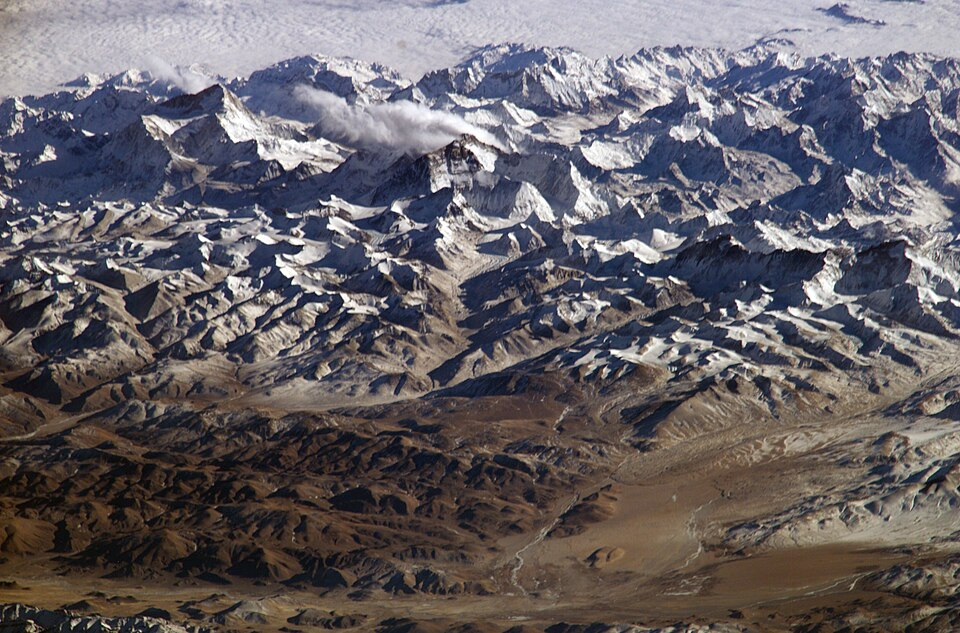
\includegraphics[width=0.75\linewidth]{images/book1/g4-himalaya-iss.jpg}

{\small De Himalaya vanuit het Internationaal Ruimtestation, met de blik
naar het zuiden vanaf het hoogland van Tibet: een \omterm{def:g2:water-on-earth:ocean}{zee} van besneeuwde
toppen. Foto: NASA (publiek domein).}
% ledger: nasa:himalaya-iss
\end{omfigure}

\section{De grote rivieren en meren}

\omterm{def:g4:clouds-rain-snow:precipitation}{Regen} en gesmolten \omterm{def:g4:clouds-rain-snow:precipitation}{sneeuw} stromen van het land, komen samen in beken en
daarna in \omterm{def:g1:landscapes-around-us:water}{rivieren}, en de \omterm{def:g1:landscapes-around-us:water}{rivieren} voeren het water naar beneden, naar de
\omterm{def:g2:water-on-earth:ocean}{zee}. De grootste \omterm{def:g1:landscapes-around-us:water}{rivieren} voeren het water van hele delen van een \omterm{def:g3:continents-and-oceans:continent}{continent}
af.

De twee langste \omterm{def:g1:landscapes-around-us:water}{rivieren} op Aarde zijn de Nijl, in Afrika, en de Amazone,
in Zuid-Amerika. Elk is bijna 7\,000 kilometer lang. Welke is de langste?
Niemand weet het zeker, want het hangt ervan af waar je vindt dat een
\omterm{def:g1:landscapes-around-us:water}{rivier} begint: welke van alle beekjes die samen de \omterm{def:g1:landscapes-around-us:water}{rivier} vormen, telt als
haar echte begin? In 2007 zei een team dat de Amazone tot een verder
gelegen bron had gevolgd, dat ze ongeveer 6\,800 kilometer lang was, iets
langer dan de Nijl; veel naslagwerken noemen nog steeds de Nijl de
langste.
% ledger: natgeo:nile, natgeo:amazon-nile-2007

De Amazone is zonder enige twijfel de grootste \omterm{def:g1:landscapes-around-us:water}{rivier}: ze voert meer water
af dan welke andere \omterm{def:g1:landscapes-around-us:water}{rivier} ook.
% ledger: natgeo:amazon-nile-2007

\begin{omfigure}
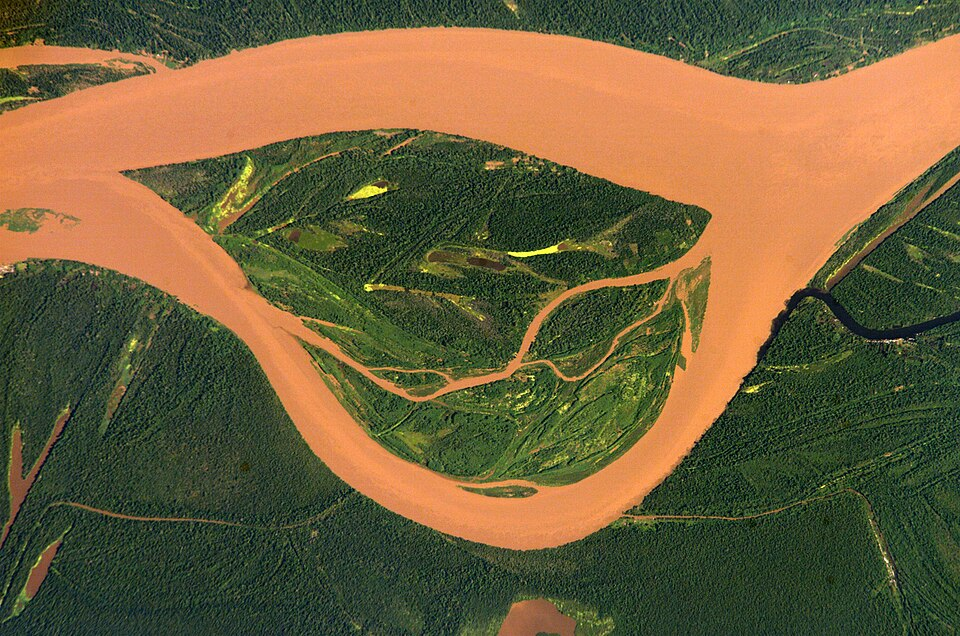
\includegraphics[width=0.6\linewidth]{images/book1/g4-amazon-iss.jpg}

{\small De Amazone, bruin van het \omterm{def:g3:stones-pebbles-sand:sand}{slib}, kronkelt door het regenwoud, gezien
vanuit het Internationaal Ruimtestation. Foto: NASA (publiek domein).}
% ledger: nasa:amazon-iss
\end{omfigure}

Ook \omterm{def:g1:landscapes-around-us:water}{meren} breken records. Het grootste meer op Aarde is de Kaspische Zee,
tussen Europa en Azië: het is zo groot dat het een \omterm{def:g2:water-on-earth:ocean}{zee} wordt genoemd, maar
het is aan alle kanten door land omsloten. Het beslaat meer dan
370\,000 vierkante kilometer. Het diepste meer is het Baikalmeer, in
Rusland: op sommige plaatsen ligt de bodem bijna 2 kilometer onder het
wateroppervlak.
% ledger: natgeo:caspian-baikal

\section{Woestijnen en het grote ijs}

Twee soorten plaatsen springen eruit op de \omterm{def:g4:world-physical-map:physical-map}{natuurkundige kaart}, omdat er
bijna niets groeit: de grote woestijnen, waar het bijna nooit regent, en
het grote ijs.

De Sahara, in het noorden van Afrika, is de grootste hete woestijn op
Aarde. Ze beslaat ongeveer achtenhalf miljoen vierkante kilometer. Heel
Afrika beslaat ongeveer 30 miljoen vierkante kilometer, dus de Sahara is
iets meer dan een kwart van het \omterm{def:g3:continents-and-oceans:continent}{continent}: meer dan $\frac{1}{4}$, maar
minder dan $\frac{1}{3}$.
% ledger: natgeo:sahara, data:etopo1

Het grote ijs bedekt Antarctica, rond de \omterm{def:g3:continents-and-oceans:poles}{Zuidpool}, en het grootste deel van
Groenland, in het hoge noorden van de Atlantische \omterm{def:g2:water-on-earth:ocean}{Oceaan}. Daar heeft de
\omterm{def:g4:clouds-rain-snow:precipitation}{sneeuw} van duizenden jaren zich opgestapeld en is ze veranderd in een dikke
laag ijs. Op de \omterm{def:g4:world-physical-map:physical-map}{natuurkundige kaart} hebben ze de kleuren van hoog land,
omdat de bovenkant van het ijs hoog boven \omterm{def:g4:world-physical-map:altitude}{zeeniveau} ligt.

\section{Het hoogste en het diepste}

De \omterm{def:g4:world-physical-map:physical-map}{natuurkundige kaart} laat de vorm van het aardoppervlak zien, maar ze is
zo klein dat ze de uitersten verbergt. Laten we die naast elkaar zetten, op
schaal.

\begin{omfigure}
\begin{tikzpicture}[x=1cm, y=0.32cm, font=\small]
  % sea level
  \fill[omHypsSeaA] (0,0) rectangle (9,-11.5);
  \fill[omHypsSeaD!80] (4.6,-11.5) -- (4.6,-11.0) -- (5.0,-10.98) -- (5.4,-11.0) -- (5.4,-11.5) -- cycle;
  \draw[black!60] (-0.2,0) -- (9.2,0);
  \node[anchor=west, font=\scriptsize] at (9.25,0) {zeeniveau, 0\,m};
  % height scale
  \draw[black!60] (0,-11.5) -- (0,10);
  \foreach \h in {-10,-8,...,8} {
    \draw[black!60] (-0.1,\h) -- (0,\h);
    \node[anchor=east, font=\scriptsize] at (-0.12,\h) {\h\,km};
  }
  % ocean floor and trench
  \fill[brown!45] (0.05,-11.5) -- (0.05,-3.7) -- (3.2,-3.7) -- (4.4,-6) -- (4.9,-10.98) -- (5.1,-10.98)
    -- (5.6,-6) -- (6.4,-3.7) -- (9,-3.7) -- (9,-11.5) -- cycle;
  \node[font=\scriptsize, align=center] at (2.0,-5.3) {oceaanbodem,\\ongeveer 3\,700\,m diep};
  \node[font=\scriptsize, anchor=west, align=left] at (5.6,-9.4) {het diepste punt:\\de Challengerdiepte,\\bijna 11\,000\,m};
  % Everest
  \fill[black!35] (6.6,0) -- (7.6,8.85) -- (8.6,0) -- cycle;
  \fill[white, draw=black!45, line width=0.3pt] (7.35,6.6) -- (7.6,8.85) -- (7.85,6.6) -- (7.6,7.1) -- cycle;
  \node[font=\scriptsize, align=center, anchor=south] at (7.6,8.95) {Mount Everest, 8\,849\,m};
  % cirrus clouds band
  \draw[black!45, line width=0.6pt] (1.0,9.0) .. controls (1.6,9.5) and (2.2,9.1) .. (2.8,9.6);
  \draw[black!45, line width=0.6pt] (1.2,8.3) .. controls (1.8,8.8) and (2.4,8.4) .. (3.0,8.9);
  \node[font=\scriptsize, align=center] at (2.0,7.2) {hoge wolken\\(cirrus)};
  % a village
  \fill[black!60] (2.2,1.5) rectangle (2.45,1.75);
  \node[font=\scriptsize, anchor=west] at (2.5,1.6) {een bergdorp, 1\,500\,m};
\end{tikzpicture}

{\small Van het diepste punt van de \omterm{def:g2:water-on-earth:ocean}{oceaan} tot de hoogste top, op schaal.
De Challengerdiepte, in de Stille \omterm{def:g2:water-on-earth:ocean}{Oceaan}, ligt dieper onder de \omterm{def:g2:water-on-earth:ocean}{zee} dan
Mount Everest erboven uitsteekt. Waarden: Everest 8\,849\,m; de
Challengerdiepte bijna 11\,000\,m; de gemiddelde oceaanbodem ongeveer
3\,700\,m.}
\label{fig:g4:world-physical-map:extremes}
% ledger: tht:everest, usgs:trench-depth, nos:ocean-depth, wmo:cloud-levels
\end{omfigure}

\begin{example}[Everest in de diepte]\label{ex:g4:world-physical-map:everest-in-deep}
Als we Mount Everest konden optillen en op de bodem van de Challengerdiepte
neerzetten, zou de top nog steeds onder water liggen: ongeveer 11\,000
meter trog tegen 8\,849 meter \omterm{def:g1:landscapes-around-us:landform}{berg}. Er zou nog meer dan 2 kilometer \omterm{def:g2:water-on-earth:ocean}{zee}
boven staan.
% ledger: tht:everest, usgs:trench-depth
\end{example}

\section{Oefeningen}

\begin{exercise}[$\star$]\label{exo:g4:world-physical-map:1}
Wat is de \omterm{def:g4:world-physical-map:altitude}{hoogte} van een plek? Vanaf welk niveau wordt ze gemeten?
\end{exercise}

\begin{exercise}[$\star$]\label{exo:g4:world-physical-map:2}
Geef met de \omterm{def:g2:drawing-to-map:legend}{legenda} van de \omterm{def:g4:world-physical-map:physical-map}{natuurkundige kaart} de \omterm{def:g4:world-physical-map:altitude}{hoogte} van een plek die
(a) donkergroen; (b) lichtgeel; (c) bijna wit gekleurd is.
\end{exercise}

\begin{exercise}[$\star$]\label{exo:g4:world-physical-map:3}
Op welk \omterm{def:g3:continents-and-oceans:continent}{continent} liggen: (a) de Andes; (b) de Himalaya; (c) de Sahara;
(d) de Rocky Mountains?
\end{exercise}

\begin{exercise}[$\star$]\label{exo:g4:world-physical-map:4}
Noem de hoogste \omterm{def:g1:landscapes-around-us:landform}{berg} op Aarde, het grootste meer en het diepste meer.
\end{exercise}

\begin{exercise}[$\star$]\label{exo:g4:world-physical-map:5}
Op de \omterm{def:g4:world-physical-map:physical-map}{natuurkundige kaart} is de \omterm{def:g2:water-on-earth:ocean}{zee} bij de \omterm{def:g1:landscapes-around-us:water}{kusten} lichtblauw en het midden
van de \omterm{def:g2:water-on-earth:ocean}{oceanen} donkerblauw. Wat zegt dat over de diepte van de \omterm{def:g2:water-on-earth:ocean}{zee}?
\end{exercise}

\begin{exercise}[$\star$]\label{exo:g4:world-physical-map:6}
Waarom hebben Antarctica en Groenland op de \omterm{def:g4:world-physical-map:physical-map}{natuurkundige kaart} de kleur
van hoog land?
\end{exercise}

\begin{exercise}[$\star\star$]\label{exo:g4:world-physical-map:7}
Zet op volgorde, van laag naar hoog: een strand; een dorp op
1\,500 meter; de top van Mount Everest; de bodem van de Challengerdiepte;
de gemiddelde oceaanbodem.
\end{exercise}

\begin{exercise}[$\star\star$]\label{exo:g4:world-physical-map:8}
Waarom kunnen we niet zeker zeggen of de Nijl of de Amazone de langste
\omterm{def:g1:landscapes-around-us:water}{rivier} is?
\end{exercise}

\begin{exercise}[$\star\star$]\label{exo:g4:world-physical-map:9}
Afrika beslaat ongeveer 30 miljoen vierkante kilometer. Hoeveel is een
kwart daarvan? En een derde? De Sahara beslaat ongeveer achtenhalf miljoen
vierkante kilometer: is dat meer of minder dan een kwart van Afrika? Meer
of minder dan een derde?
\end{exercise}

\begin{exercise}[$\star\star$]\label{exo:g4:world-physical-map:10}
Een berghut staat op 2\,500 meter, en een \omterm{def:g1:landscapes-around-us:water}{meer} eronder op 1\,000 meter.
Hoeveel meter hoger ligt de hut? Welke kleuren hebben ze op de
\omterm{def:g4:world-physical-map:physical-map}{natuurkundige kaart}?
\end{exercise}

\begin{exercise}[$\star\star\star$]\label{exo:g4:world-physical-map:11}
Een vliegtuig vliegt 10 kilometer boven \omterm{def:g4:world-physical-map:altitude}{zeeniveau}. Vliegt het hoger dan
Mount Everest? Hoeveel meter? Als het boven de Challengerdiepte vloog, hoe
ver zou het dan boven de bodem van de trog zijn (neem 11\,000 meter voor de
trog)?
\end{exercise}
